\chapter{Moti piani}
Un moto piano di un corpo rigido è caratterizzato dai vincoli
\[
\omega_x=\omega_y=0
\]
\[
z_p=k\in\mathbb{R}\qquad \forall\, p \in\mathcal{R}
\]

In particolare mostriamo che i vincoli olonomi
\[
\omega_x=\omega_y=0
\]
\[
z_q=0,\qquad q\in\mathcal{R}
\]
bastano per descrivere il sistema. Sia $p$ un punto del corpo rigido che ha componente $z_p=0$ nel nostro sistema di riferimento scelto. Sia $q$ un altro punto del corpo rigido. Mostriamo che $z_q=k\in\mathbb{R}$. Impostando la legge fondamentale si ottiene
\[
\underline{v}_q=\underline{v}_p+\underline{\omega}\wedge(\underline{x}_q-\underline{x}_p)
\]
e applicando i vincoli $z_p=0$, $\omega_x=\omega_y=0$ si ha
\[
\underline{\omega}=
\begin{pmatrix}
0\\
0\\
\omega_z
\end{pmatrix},
\qquad
\underline{x}_p=
\begin{pmatrix}
x_p\\
y_p\\
0
\end{pmatrix},
\qquad
\underline{x}_q=
\begin{pmatrix}
x_q\\
y_q\\
z_q
\end{pmatrix}
\]
\[
\underline{v}_p=
\begin{pmatrix}
v_{p,x}\\
v_{p,y}\\
0
\end{pmatrix},
\qquad
\underline{v}_q=
\begin{pmatrix}
v_{q,x}\\
v_{q,y}\\
v_{q,z}
\end{pmatrix}
\]
da cui
\[
\underline{v}_q=
\begin{pmatrix}
v_{q,x}\\
v_{q,y}\\
v_{q,z}
\end{pmatrix}
=
\begin{pmatrix}
v_{p,x}\\
v_{p,y}\\
0
\end{pmatrix}
+
\begin{pmatrix}
0\\
0\\
\omega_z
\end{pmatrix}
\wedge
\begin{pmatrix}
x_q-x_p\\
y_q-y_p\\
z_q
\end{pmatrix}
=
\]
\[
=
\begin{pmatrix}
v_{p,x}\\
v_{p,y}\\
0
\end{pmatrix}
+
\begin{vmatrix}
\hat{\imath} & \hat{\jmath} & \hat{k}\\
0 & 0 & \omega_z\\
x_q-x_p & y_q-y_p & z_q
\end{vmatrix}
=
\begin{pmatrix}
v_{p,x}\\
v_{p,y}\\
0
\end{pmatrix}
+\hat{\imath}\bigl(-\omega_z(y_q-y_p)\bigr)
+\hat{\jmath}\bigl(\omega_z(x_q-x_p)\bigr)
+\hat{k}\cdot 0
\]
\[
=
\begin{pmatrix}
v_{p,x}\\
v_{p,y}\\
0
\end{pmatrix}
+
\begin{pmatrix}
\omega_z y_p-\omega_z y_q\\
\omega_z x_q-\omega_z x_p\\
0
\end{pmatrix}
=
\begin{pmatrix}
v_{p,x}+\omega_z y_p-\omega_z y_q\\
v_{p,y}+\omega_z x_q-\omega_z x_p\\
0
\end{pmatrix}.
\]

In particolare
\[
v_{q,z}=0 \;\;\Rightarrow\;\; z_q=k\in\mathbb{R}.
\]
Un corpo rigido vincolato ad un moto piano ha quindi $6-3=3$ gradi di libertà.\\
Possiamo ad esempio descriverlo attraverso le coordinate libere
\[
x_{p}(t) , y_{p}(t) , w_z(t)  \quad p \in \mathcal{R}
\]

\begin{examplebreak}{}
Consideriamo un'asta rigida con un estremo $O$ vincolato nell'origine degli assi e costretto ad un moto piano.

\begin{figure}
\begin{tikzpicture}[scale=1.2]
    % assi
    \draw[->] (0,-3.2) -- (0,1.2) node[above] {$y$};
    \draw[->] (-0.2,0) -- (3.4,0) node[right] {$x$};

    % origine
    \fill (0,0) circle (2pt);
    \node[below left] at (0,0) {$O$};

    % asta
    \coordinate (P) at (1.55,-2.35);
    \draw[line width=0.9pt] (0,0) -- (P);

    % punto P
    \fill (P) circle (2pt);
    \node[right] at (P) {$P$};

    % arco theta
    \draw[->] (0,-1.15) arc[start angle=-90,end angle=-56,radius=1.15];
    \node[left] at (0.33,-1.45) {$\theta$};

    % arco l

    \node[right] at (1.1,-1.05) {$l$};

    % velocità vp
    \draw[->,red,line width=0.9pt] (P) -- ++(1.2,0.75);
    \node[red,right] at (2.75,-1.58) {$\underline{v}_p$};
\end{tikzpicture}
\end{figure}

Oltre ai vincoli del moto piano possiamo impostare
\[
x_O(t)=y_O(t)=0.
\]

Il corpo rigido ha quindi $3-2=1$ grado di libertà. Scegliamo come coordinata libera $\theta(t)$, l'angolo formato dall'asta con l'asse $y$, come illustrato in figura.

Impostiamo la legge fondamentale con $q=O$, da cui
\[
\underline{x}_q=
\begin{pmatrix}
0\\
0\\
0
\end{pmatrix},
\qquad
\underline{v}_q=\underline{0},
\]
e quindi
\[
\underline{v}_p=\underline{v}_q+\underline{\omega}\wedge(\underline{x}_p-\underline{x}_q)
=\underline{\omega}\wedge \underline{x}_p.
\]

Tenendo in considerazione che
\[
\underline{\omega}=
\begin{pmatrix}
0\\
0\\
\dot{\theta}
\end{pmatrix},
\qquad
\underline{x}_p=
\begin{pmatrix}
x_p\\
y_p\\
0
\end{pmatrix},
\]
allora
\[
\underline{v}_p=
\begin{pmatrix}
0\\
0\\
\dot{\theta}
\end{pmatrix}
\wedge
\begin{pmatrix}
x_p\\
y_p\\
0
\end{pmatrix}
=
\begin{vmatrix}
\hat{\imath} & \hat{\jmath} & \hat{k}\\
0 & 0 & \dot{\theta}\\
x_p & y_p & 0
\end{vmatrix}
=
\hat{\imath}(-y_p\dot{\theta})-\hat{\jmath}(-x_p\dot{\theta}),
\]
cioè
\[
\underline{v}_p=
\begin{pmatrix}
-y_p\dot{\theta}\\
x_p\dot{\theta}\\
0
\end{pmatrix}.
\]

Pertanto
\[
\underline{v}_p=(-y_p\dot{\theta},\,x_p\dot{\theta},\,0)^T
=
\|\underline{\omega}\|\,\|\underline{x}_p\|\,\hat{u}_{\perp}
=
l\,|\dot{\theta}|\,\hat{u}_{\perp},
\]
dove nell'ultimo passaggio
\[
l=\left\|
\begin{pmatrix}
x_p\\
y_p
\end{pmatrix}
\right\|
=d\!\left(
\begin{pmatrix}
x_p\\
y_p
\end{pmatrix},
\underline{0}\right)
\]
è costante perché il corpo è rigido e vincolato.

Nel penultimo passaggio abbiamo usato la regola della mano destra e la relazione
\[
\|\underline{v}_1\wedge \underline{v}_2\|
=
\|\underline{v}_1\|\,\|\underline{v}_2\|\sin\varphi.
\]
\end{examplebreak}
\begin{examplebreak}{}
Consideriamo ora una situazione fisica simile al precedente esempio. Questa volta però l'estremo $O$ dell'asta non è vincolato nell'origine degli assi, ma è mobile su una guida orizzontale posta lungo l'asse $x$.

\begin{figure}
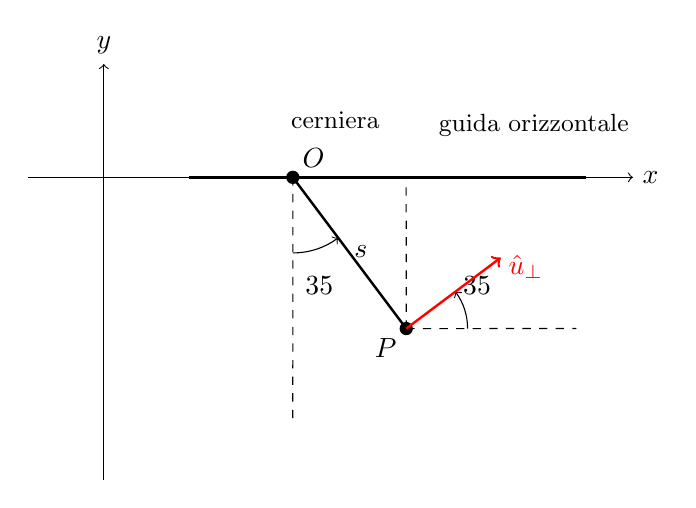
\begin{tikzpicture}[scale=1.2]
    % assi
    \draw[->] (-0.8,0) -- (5.6,0) node[right] {$x$};
    \draw[->] (0,-3.2) -- (0,1.2) node[above] {$y$};

    % guida orizzontale
    \draw[line width=0.9pt] (0.9,0) -- (5.1,0);
    \node at (4.55,0.55) {\small guida orizzontale};

    % punto O
    \coordinate (O) at (2.0,0);
    \fill (O) circle (2pt);
    \node[above right] at (O) {$O$};

    % punto P
    \coordinate (P) at (3.2,-1.6);
    \fill (P) circle (2pt);
    \node[below left] at (P) {$P$};

    % asta
    \draw[line width=0.9pt] (O) -- (P);

    % proiezioni tratteggiate
    \draw[dashed] (O) -- (2.0,-2.6);
    \draw[dashed] (P) -- (3.2,0);
    \draw[dashed] (P) -- (5.0,-1.6);

    % etichetta s
    \node at (2.72,-0.78) {$s$};

    % arco theta a sinistra
    \draw[->] (2.0,-0.8) arc[start angle=-90,end angle=-53,radius=0.8];
    \node at (2.28,-1.15) {$\theta$};

    % arco theta a destra
    \draw[->] (3.85,-1.6) arc[start angle=0,end angle=37,radius=0.65];
    \node at (3.95,-1.15) {$\theta$};

    % velocità
    \draw[->,red,line width=0.9pt] (P) -- ++(1.0,0.75);
    \node[red,right] at (4.18,-0.95) {$\hat{u}_\perp$};

    % etichette varie
    \node at (2.45,0.6) {\small cerniera};
\end{tikzpicture}
\end{figure}

L'asta è soggetta quindi ai vincoli del moto piano e al vincolo
\[
y_O(t)=0.
\]

Ha dunque $3-1=2$ gradi di libertà. Usiamo le coordinate libere $x_O(t)$ e $\theta(t)$, ovvero la posizione lungo l'asse $x$ di $O$ e l'angolo $\theta(t)$ analogo all'esempio precedente.

Supponiamo $x_O(t)$ e $\theta(t)$ noti. Determiniamo $\underline{v}_p(t)$ per ogni $p$ e per ogni $t$.

Per la legge fondamentale della cinematica del corpo rigido,
\[
\underline{v}_p(t)=\underline{v}_O+\underline{\omega}\wedge(\underline{x}_p-\underline{x}_O).
\]

Poiché il moto è piano,
\[
\underline{\omega}=
\begin{pmatrix}
0\\
0\\
\dot{\theta}(t)
\end{pmatrix},
\qquad
\underline{v}_O=
\begin{pmatrix}
\dot{x}_O(t)\\
0\\
0
\end{pmatrix}.
\]

Inoltre
\[
\underline{x}_p-\underline{x}_O=
\begin{pmatrix}
x_p-x_O\\
y_p\\
0
\end{pmatrix}.
\]

Allora
\[
\underline{v}_p(t)=
\begin{pmatrix}
\dot{x}_O(t)\\
0\\
0
\end{pmatrix}
+
\begin{pmatrix}
0\\
0\\
\dot{\theta}(t)
\end{pmatrix}
\wedge
\begin{pmatrix}
x_p-x_O\\
y_p\\
0
\end{pmatrix}.
\]

Sviluppando il prodotto vettoriale,
\[
\underline{v}_p(t)=
\begin{pmatrix}
\dot{x}_O(t)\\
0\\
0
\end{pmatrix}
+
\begin{vmatrix}
\hat{\imath} & \hat{\jmath} & \hat{k}\\
0 & 0 & \dot{\theta}(t)\\
x_p-x_O & y_p & 0
\end{vmatrix}
=
\begin{pmatrix}
\dot{x}_O(t)-y_p\dot{\theta}(t)\\
(x_p-x_O)\dot{\theta}(t)\\
0
\end{pmatrix}.
\]

Quindi
\[
\underline{v}_p(t)
=
\dot{x}_O(t)\,\hat{\imath}
-y_p\dot{\theta}(t)\,\hat{\imath}
+(x_p-x_O)\dot{\theta}(t)\,\hat{\jmath}.
\]

Se indichiamo con
\[
s=
d\!\left(
\begin{pmatrix}
x_p\\
y_p
\end{pmatrix},
\begin{pmatrix}
x_O\\
0
\end{pmatrix}
\right)
\]
la distanza tra $P$ e $O$, che è costante perché l'asta è rigida, allora il termine rotazionale può essere scritto come
\[
s\,\dot{\theta}\,\hat{u}_\perp.
\]

Pertanto si ottiene
\[
\underline{v}_p(t)=\dot{x}_O(t)\,\hat{\imath}+s\,\dot{\theta}\,\hat{u}_\perp.
\]
\end{examplebreak}

\section{Moto di puro rotolamento}
\begin{definition}{}
Diciamo che due corpi rigidi che sono in contatto in un punto $P$ sono sottoposti ad un \emph{vincolo di puro rotolamento} se
\[
{}^{1}\underline{v}_P(t) = {}^{2}\underline{v}_P(t),
\]
dove ${}^{1}\underline{v}_P(t)$ è la velocità del punto di contatto $P$ vista dal corpo $1$ e ${}^{2}\underline{v}_P(t)$ è la velocità dello stesso punto vista dal corpo $2$.
\end{definition}

\begin{oss}{}
\begin{center}
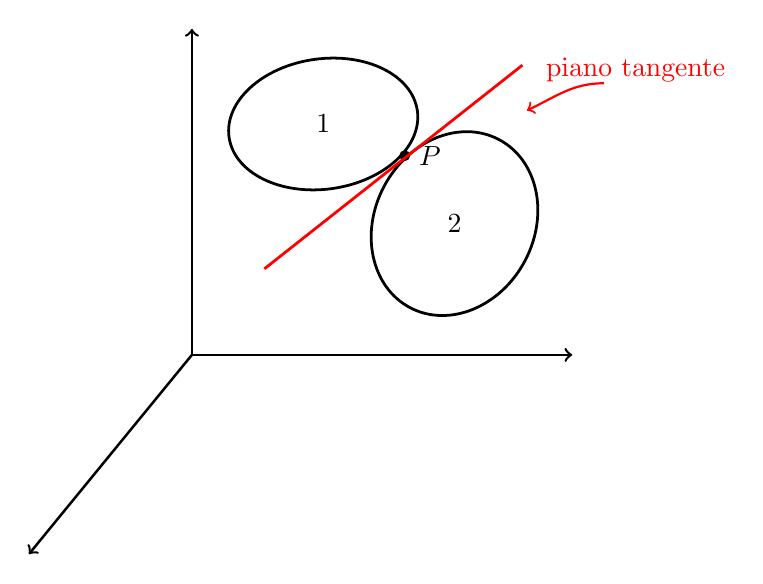
\begin{tikzpicture}[scale=1.15]

% terna cartesiana
\draw[->, line width=0.9pt] (0,0) -- (4.2,0);
\draw[->, line width=0.9pt] (0,0) -- (0,3.6);
\draw[->, line width=0.9pt] (0,0) -- (-1.8,-2.2);

% corpi rigidi stilizzati
\draw[line width=1pt] (1.45,2.55) ellipse [x radius=1.05, y radius=0.72, rotate=8];
\draw[line width=1pt] (2.9,1.45) ellipse [x radius=0.88, y radius=1.05, rotate=-28];

% punto di contatto
\fill (2.35,2.2) circle (1.7pt);
\node[right] at (2.4,2.2) {$P$};

% etichette corpi
\node at (1.45,2.55) {$1$};
\node at (2.9,1.45) {$2$};

% piano tangente (rappresentato da una retta nel disegno)
\draw[red, line width=1pt] (0.8,0.95) -- (3.65,3.2);
\node[red] at (4.9,3.15) {piano tangente};
\draw[red,->,line width=0.8pt] (4.55,3.0) to[out=180,in=25] (3.7,2.7);

\end{tikzpicture}
\end{center}

In un punto di contatto $P$ fra due corpi rigidi, le componenti delle velocità dei due corpi perpendicolari al piano tangente in $P$ devono essere concordi. In caso contrario, i due corpi tenderebbero a compenetrarsi, il che è incompatibile con il vincolo di contatto.
\end{oss}

\begin{examplebreak}{}
Moto di un disco in un piano orizzontale fermo.

\begin{figure}
\centering
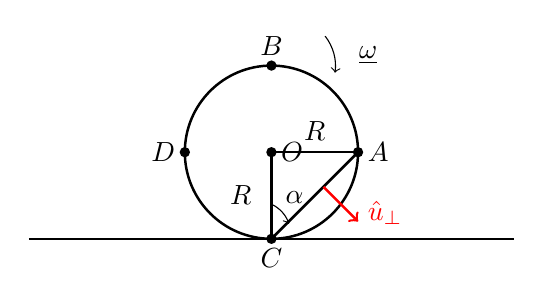
\begin{tikzpicture}[scale=1.1]
    % piano
    \draw[line width=0.9pt] (-2.8,0) -- (2.8,0);

    % disco
    \draw[line width=0.9pt] (0,1) circle (1);

    % punti
    \fill (0,1) circle (1.7pt);
    \fill (1,1) circle (1.7pt);
    \fill (0,0) circle (1.7pt);
    \fill (0,2) circle (1.7pt);
    \fill (-1,1) circle (1.7pt);

    \node[right] at (0,1) {$O$};
    \node[right] at (1,1) {$A$};
    \node[below] at (0,0) {$C$};
    \node[above] at (0,2) {$B$};
    \node[left] at (-1,1) {$D$};

    % raggi
    \draw[line width=0.9pt] (0,1) -- (1,1);
    \draw[line width=0.9pt] (0,1) -- (0,0);
    \draw[line width=0.9pt] (0,0) -- (1,1);

    % etichette
    \node[left] at (-0.12,0.5) {$R$};
    \node[above] at (0.5,1.02) {$R$};

    % angolo alpha
    \draw[->] (0,0.4) arc[start angle=65,end angle=18,radius=0.38];
    \node[right] at (0.05,0.48) {$\alpha$};

    % omega
    \draw[->] (0.62,2.34) arc[start angle=38,end angle=-8,radius=0.56];
    \node[right] at (0.9,2.12) {$\underline{\omega}$};

    % u_perp
    \draw[->,red,line width=0.9pt] (0.6,0.6) -- (1,0.2);
    \node[red,right] at (1,0.3) {$\hat{u}_{\perp}$};
\end{tikzpicture}
\end{figure}

Chiamiamo $C$ il punto di contatto con il piano al tempo $t$.

Impongo $\underline{v}_C(t)=0$. Toglie $2$ gradi di libertà e ne resta $1$.

Descriviamo il moto usando
\[
\underline{\omega}=\dot{\theta}\,\hat{k}.
\]

Definisco $\underline{\omega}$ positivo in senso orario (uso $(0,0,-1)^T$
nella base).

Scelgo di utilizzare la formula fondamentale del moto dei corpi rigidi con $x_q=x_C$.
Sotto ipotesi di puro rotolamento $\underline{v}_C=(0,0,0)$.
Calcoliamo la velocità di $O$.
\[
\underline{v}_O=0+R\dot{\theta}\,\hat{\imath}
\qquad
\underline{v}_B=0+2R\dot{\theta}\,\hat{\imath}
\]

\[
\underline{v}_A=\underline{v}_O+\underline{\omega}\wedge(\underline{x}_A-\underline{x}_O)
=R\dot{\theta}\,\hat{\imath}-\dot{\theta}R\,\hat{\jmath}
=\dot{\theta}R(\hat{\imath}-\hat{\jmath})
=
\dot{\theta}R
\begin{pmatrix}
1\\
-1\\
0
\end{pmatrix}
\]
\[
\underline{v}_D=R\dot{\theta}\,\hat{\imath}+R\dot{\theta}\,\hat{\jmath}
=
R\dot{\theta}
\begin{pmatrix}
1\\
1\\
0
\end{pmatrix}
\]

Possiamo anche calcolare $\underline{v}_A$ a partire da $C$.
\[
\underline{v}_A=
\underline{\omega}\wedge(\underline{x}_A-\underline{x}_C)
=
-\frac{R}{\sin\alpha}\,\dot{\theta}\,\hat{\jmath}
=
\sqrt{2}\,R\dot{\theta}\,\hat{u}_{\perp}
=
\sqrt{2}\,R\dot{\theta}
\begin{pmatrix}
\frac{1}{\sqrt{2}}\\[4pt]
-\frac{1}{\sqrt{2}}\\[4pt]
0
\end{pmatrix}
=
R\dot{\theta}
\begin{pmatrix}
1\\
-1\\
0
\end{pmatrix}
\]
\end{examplebreak}

\begin{examplebreak}{}
Consideriamo un disco che rotola senza strisciare su un carrello che trasla orizzontalmente.

\begin{figure}
\begin{tikzpicture}[scale=1.15]
    % assi
    \draw[->] (-0.3,0) -- (6.4,0) node[right] {$x$};
    \draw[->] (0,-0.3) -- (0,3.8) node[above] {$y$};

    % carrello appoggiato sull'asse x
    \draw[line width=0.9pt] (1.2,0) -- (5.4,0);
    \fill (1.5,0) circle (1.6pt);
    \fill (5.1,0) circle (1.6pt);
    \node[above] at (1.5,0) {$A$};
    \node[above] at (5.1,0) {$B$};

    % piedini/ruote simmetrici e dritti sotto il carrello
    \draw[line width=0.9pt] (2.2,0) -- (2.05,-0.22) -- (2.35,-0.22) -- cycle;
    \draw[line width=0.9pt] (4.2,0) -- (4.05,-0.22) -- (4.35,-0.22) -- cycle;

    % disco tangente al carrello
    \def\R{1}
    \coordinate (C) at (3.3,0);
    \coordinate (O) at (3.3,1.0);
    \draw[line width=0.9pt] (O) circle (\R);

    % centro e punto di contatto
    \fill (O) circle (1.5pt);
    \fill (C) circle (1.5pt);
    \node[right] at (3.35,1.02) {$O$};
    \node[below] at (3.3,-0.02) {$C$};
\end{tikzpicture}
\end{figure}

Abbiamo due corpi rigidi, quindi in totale $6$ gradi di libertà.

I vincoli sono:
\[
y_A=0,\qquad y_B=0,
\]
e il vincolo di puro rotolamento nel punto di contatto $C$,
\[
\underline{v}_C^{\text{disco}}=\underline{v}_C^{\text{carrello}}.
\]

In totale otteniamo $4$ vincoli, dunque rimangono
\[
6-4=2
\]
gradi di libertà.

Scegliamo come coordinate libere
\[
x_A,\qquad \theta.
\]

Applicando la formula fondamentale della cinematica del corpo rigido al disco, con polo in $C$, si ha
\[
\underline{v}_O=\underline{v}_C+\underline{\omega}\wedge(\underline{x}_O-\underline{x}_C).
\]
Poiché il carrello trasla orizzontalmente,
\[
\underline{v}_C=\dot{x}_A\,\hat{\imath},
\]
mentre, essendo
\[
\underline{\omega}=\dot{\theta}\,\hat{k},
\qquad
\underline{x}_O-\underline{x}_C=R\,\hat{\jmath},
\]
segue
\[
\underline{v}_O=\dot{x}_A\,\hat{\imath}+\dot{\theta}\,\hat{k}\wedge R\,\hat{\jmath}
=\dot{x}_A\,\hat{\imath}+R\dot{\theta}\,\hat{\imath}.
\]
Quindi
\[
\underline{v}_O=(\dot{x}_A+R\dot{\theta})\,\hat{\imath}.
\]
\end{examplebreak}

\begin{oss}{}
Il vincolo di puro rotolamento in questo caso è integrabile.
\end{oss}
\begin{oss}{}
    Sull'asse verticale del disco la velocità dovuta al puro rotolamento aumenta linearmente con la distanza da C.
    \begin{center}
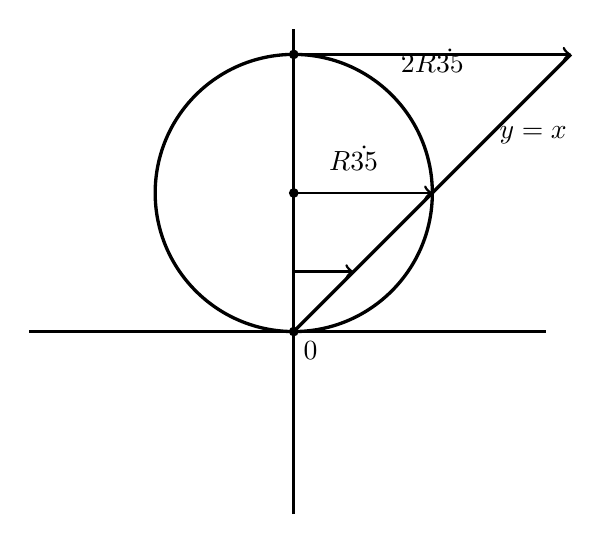
\begin{tikzpicture}[scale=0.8]
    % parametri
    \def\R{2.2}
    \pgfmathsetmacro{\rt}{sqrt(2)*\R}

    % piano orizzontale
    \draw[line width=1.1pt] (-4.2,0) -- (4.0,0);

    % asse verticale
    \draw[line width=1.1pt] (0,-2.9) -- (0,4.8);

    % disco
    \draw[line width=1.2pt] (0,\R) circle (\R);

    % punti notevoli
    \fill (0,0) circle (2.2pt);
    \node[below right] at (0,0) {$0$};

    \fill (0,\R) circle (2.2pt);
    \fill (0,2*\R) circle (2.2pt);

    % retta obliqua
    \draw[line width=1.2pt] (0,0) -- ({\R * 2},{\R * 2});
    \node[right] at (\rt,\rt) {$y=x$};



    % frecce orizzontali
    \draw[->, line width=1pt] (0,0.95) -- (0.95,0.95);
    \draw[->, line width=1pt] (0,\R) -- ({\R},{\R});
    \draw[->, line width=1pt] (0,{\R * 2}) -- ({\R * 2},{\R * 2});

    % etichette
    \node at (0.95,\R+0.55) {$R\dot{\theta}$};
    \node[above] at (2.2,3.95) {$2R\dot{\theta}$};
\end{tikzpicture}
\end{center}
\end{oss}

\begin{theorem}{}
    La velocità angolare   è univocamente determinata dal moto del corpo rigido. In particolare non cambia da punto a punto del corpo rigido.
\end{theorem}
\begin{proof}
Siano $\underline{\omega}_1$ e $\underline{\omega}_2$ due vettori velocità angolare associati allo stesso atto di moto, valutati a partire da due poli di riferimento diversi $q_1$ e $q_2$.

Per un generico punto $p$ del corpo rigido possiamo scrivere:
\[
\underline{v}_p=\underline{v}_{q_1}+\underline{\omega}_1\wedge(\underline{x}_p-\underline{x}_{q_1})
\]
\[
\underline{v}_p=\underline{v}_{q_2}+\underline{\omega}_2\wedge(\underline{x}_p-\underline{x}_{q_2})
\]

Sottraiamo le 2 equazioni:
\[
\underline{0}=\underline{v}_{q_1}-\underline{v}_{q_2}
+\underline{\omega}_1\wedge(\underline{x}_p-\underline{x}_{q_1})
-\underline{\omega}_2\wedge(\underline{x}_p-\underline{x}_{q_2})
\]

Esprimiamo $\underline{v}_{q_2}$ rispetto a $q_1$ tramite la formula fondamentale:
\[
\underline{v}_{q_2}=\underline{v}_{q_1}+\underline{\omega}_1\wedge(\underline{x}_{q_2}-\underline{x}_{q_1})
\]

Sostituendo nell'espressione precedente:
\[
\underline{0}
=
\underline{v}_{q_1}
-
\Bigl(\underline{v}_{q_1}+\underline{\omega}_1\wedge(\underline{x}_{q_2}-\underline{x}_{q_1})\Bigr)
+\underline{\omega}_1\wedge(\underline{x}_p-\underline{x}_{q_1})
-\underline{\omega}_2\wedge(\underline{x}_p-\underline{x}_{q_2})
\]

Sviluppando i prodotti vettoriali:
\[
\Rightarrow\quad
\underline{0}
=
-\underline{\omega}_1\wedge \underline{x}_{q_2}
+\underline{\omega}_1\wedge \underline{x}_{q_1}
+\underline{\omega}_1\wedge \underline{x}_p
-\underline{\omega}_1\wedge \underline{x}_{q_1}
-\underline{\omega}_2\wedge \underline{x}_p
+\underline{\omega}_2\wedge \underline{x}_{q_2}
\]

Semplificando i termini opposti:
\[
\Rightarrow\quad
\underline{0}
=
-\underline{\omega}_1\wedge \underline{x}_{q_2}
+\underline{\omega}_1\wedge \underline{x}_p
-\underline{\omega}_2\wedge \underline{x}_p
+\underline{\omega}_2\wedge \underline{x}_{q_2}
\]

Raccogliendo a fattor comune i prodotti vettoriali:
\[
\Rightarrow\quad
\underline{0}
=
\underline{\omega}_1\wedge(\underline{x}_p-\underline{x}_{q_2})
-\underline{\omega}_2\wedge(\underline{x}_p-\underline{x}_{q_2})
\]

\[
\Rightarrow\quad
\underline{0}
=
(\underline{\omega}_1-\underline{\omega}_2)\wedge(\underline{x}_p-\underline{x}_{q_2})
\qquad \forall\,\underline{x}_p
\]

Poiché questa relazione deve valere per ogni punto $p$, e quindi per un generico vettore $(\underline{x}_p-\underline{x}_{q_2})$, l'unica soluzione possibile affinché il prodotto vettoriale sia sempre nullo è che il primo fattore sia nullo:
\[
\Rightarrow\quad
\underline{\omega}_1-\underline{\omega}_2=0
\iff
\underline{\omega}_1=\underline{\omega}_2
\]
\end{proof}

\begin{example}{}
\begin{center}
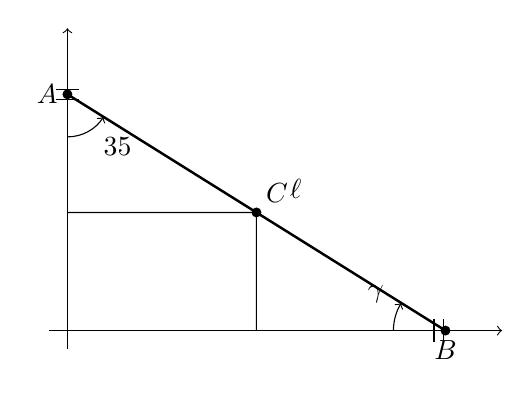
\begin{tikzpicture}[scale=1.2]
    % assi
    \draw[->] (-0.2,0) -- (4.6,0);
    \draw[->] (0,-0.2) -- (0,3.2);

    % punti
    \coordinate (A) at (0,2.5);
    \coordinate (B) at (4,0);
    \coordinate (C) at (2,1.25);

    % asta
    \draw[line width=0.9pt] (A) -- (B);

    % proiezioni di C
    \draw (C) -- (0,1.25);
    \draw (C) -- (2,0);

    % punti marcati
    \fill (A) circle (1.5pt);
    \fill (B) circle (1.5pt);
    \fill (C) circle (1.5pt);

    % etichette
    \node[left] at (A) {$A$};
    \node[below] at (B) {$B$};
    \node[above right] at (C) {$C$};
    \node[right] at (2.25,1.5) {$\ell$};

    % vincoli in A e B
    \draw (-0.12,2.55) -- (0.12,2.55);
    \draw (-0.12,2.45) -- (0.12,2.45);

    \draw (3.88,-0.12) -- (3.88,0.12);
    \draw (3.98,-0.12) -- (3.98,0.12);

    % angolo theta
    \draw[->] (0,2.05) arc[start angle=-90,end angle=-32,radius=0.45];
    \node[right] at (0.28,1.95) {$\theta$};

    % angolo gamma
    \draw[->] (3.45,0) arc[start angle=180,end angle=148,radius=0.55];
    \node[left] at (3.45,0.38) {$\gamma$};
\end{tikzpicture}
\end{center}

I vincoli sono
\[
\begin{cases}
x_A=0 \qquad \forall t,\\
y_B=0 \qquad \forall t,
\end{cases}
\]
da cui si ha $3-2 = 1$ grado di libertà.

Come coordinata libera posso scegliere:
\[
\theta(t),\ \gamma(t),\ x_B(t),\ y_A(t),\ x_C(t),\ y_C(t).
\]

Usiamo $\theta(t)$.

\[
\begin{cases}
x_C=\dfrac{\ell}{2}\sin\theta,\\[6pt]
y_C=\dfrac{\ell}{2}\cos\theta
\end{cases}
\qquad \Longrightarrow \qquad
\underline{v}_C=
\begin{pmatrix}
\dfrac{\ell}{2}\cos\theta\,\dot{\theta}\\[6pt]
-\dfrac{\ell}{2}\sin\theta\,\dot{\theta}
\end{pmatrix}.
\]
\end{example}



\begin{example}{}
    Studiamo il seguente sistema
\begin{center}
\begin{tikzpicture}[scale=0.9, >=stealth]

% parametri
\def\Rbig{3}
\def\Rsmall{1}
\def\theta{35} % angolo dal verticale verso destra

% centri (usando le coordinate polari dirette di TikZ)
\coordinate (O) at (0,0);
\coordinate (A) at ({-90+\theta}:2*\Rsmall); % distanza 2R
\coordinate (C) at ({-90+\theta}:3*\Rsmall); % distanza 3R

% circonferenza fissa
\draw[line width=1.2pt] (O) circle (\Rbig);

% disco piccolo (riempito di bianco per coprire l'asse e pulire il disegno)
\draw[line width=1.2pt, fill=white] (A) circle (\Rsmall);

% segmento OA in rosso e AC in nero
\draw[red, line width=1.2pt] (O) -- (A);
\draw[line width=1pt] (A) -- (C);

% tratteggio verticale
\draw[dashed, thick] (O) -- (0,-2.8);

% punti
\fill (O) circle (2.2pt) node[above] {$O$};
\fill (A) circle (2.2pt) node[above right, xshift=2pt] {$A$};
\fill (C) circle (2.2pt) node[below right] {$C$};

% etichetta R
\node[right] at ($(A)!0.5!(C)$) {$R$};

% --- CORREZIONE VERSORE \hat{n} ---
% Disegnato perpendicolare all'asta, con il simbolo di angolo retto
\draw[->, line width=1.1pt, purple] (A) -- ++(\theta:1.2) node[above right, inner sep=1pt] {$\hat{n}$};
% Simboletto angolo retto
\draw[line width=0.6pt] ($(A)+({-90+\theta}:0.25)$) -- ++(\theta:0.25) -- ++({90+\theta}:0.25);


% --- CORREZIONE ROTAZIONI E ANGOLO ---
% angolo theta (minuscolo, coerente col testo!)
\draw[line width=0.9pt] (0,-0.8) arc[start angle=-90, end angle={-90+\theta}, radius=0.8];
\node at ({-90+\theta/2}:0.6) {$\theta$};

% freccia Omega dell'asta (ora abbraccia la cerniera in modo fluido)
\draw[->, line width=1pt, red!80!black] (0,-1.4) arc[start angle=-90, end angle={-90+\theta-5}, radius=1.4];
\node[red!80!black, below] at ({-90+\theta/2}:1.55) {$\Omega$};

% freccia omega del disco (ruota perfettamente attorno ad A)
\draw[->, line width=1pt, green!50!black] ($(A)+({90+\theta+40}:1.3)$) arc[start angle={90+\theta+40}, end angle={90+\theta-40}, radius=1.3];
\node[green!50!black, above] at ($(A)+(90+\theta:1.4)$) {$\omega$};

\end{tikzpicture}
\end{center}


Consideriamo una guida circolare fissa di raggio $3R$.

In $C$ imponiamo il puro rotolamento.

Chiamiamo
\begin{itemize}
    \item $\omega$ velocità angolare del disco,
    \item $\Omega$ velocità angolare dell'asta.
\end{itemize}

Ad una prima analisi verrebbe da imporre i $6$ vincoli
\begin{itemize}
    \item $x_O^{\text{asta}}=y_O^{\text{asta}}=0$,
    \item $\underline{v}_C=\underline{0}$,
    \item $x_A^{\text{asta}}(t)=x_A^{\text{disco}}(t)$,
    \item $y_A^{\text{asta}}(t)=y_A^{\text{disco}}(t)$,
\end{itemize}
che però non possono essere indipendenti, perché altrimenti il sistema avrebbe $0$ gradi di libertà.

Possiamo mostrare la dipendenza riscrivendo $\underline{v}_C$ nella base del diedro di Frenet associato alla guida.

Stiamo imponendo che
\[
\underline{v}_C=0\cdot \hat{\imath}+0\cdot \hat{\jmath}
\]
e cambiando base possiamo scrivere
\[
\underline{v}_C=0\cdot \underline{T}+0\cdot \underline{N}
\]
dal momento che il vettore nullo ha coordinate $(0,0)$ in ogni base.

A questo punto notiamo che l'insieme dei vincoli
\[
x_A^{\text{asta}}(t)=x_A^{\text{disco}}(t),
\qquad
y_A^{\text{asta}}(t)=y_A^{\text{disco}}(t),
\qquad
x_O^{\text{asta}}=y_O^{\text{asta}}=0
\]
già impongono che la componente lungo $\underline{n}$ di $\underline{v}_C$ sia nulla e quindi
\[
\underline{v}_C=\underline{0}
\]
dà solo $1$ vincolo aggiuntivo.

Il sistema ha dunque
\[
6-5=1
\]
grado di libertà.

Scelgo come coordinata libera l'angolo $\theta(t)$ che l'asta forma con il diametro verticale della guida.

Notiamo che
\[
\Omega=\dot{\theta}.
\]
Dobbiamo essere in grado di ricavare anche $\omega$ in funzione di $\dot{\theta}$.

\[
\underline{v}_A^{\text{asta}}
=
\underline{v}_O+\underline{\Omega}\wedge(\underline{x}_A-\underline{x}_O)
=
0+\Omega\,2R\,\hat{n}
\]

\[
\underline{v}_A^{\text{disco}}
=
\underline{v}_C+\underline{\omega}\wedge(\underline{x}_A-\underline{x}_C)
=
0+\omega R\,\hat{n}
\]

Usando
\[
\underline{x}_A^{\text{asta}}=\underline{x}_A^{\text{disco}}
\]
si ottiene
\[
\underline{v}_A^{\text{disco}}=\underline{v}_A^{\text{asta}}
\]
e quindi
\[
\omega R=2R\,\Omega
\quad\Rightarrow\quad
\omega=2\Omega=2\dot{\theta}.
\]
\end{example}
